\documentclass{beamer}

\usepackage[utf8]{inputenc}
\usepackage{graphicx}
\usepackage{amsmath}
\usepackage{hyperref}
\usepackage{tikz}
\usepackage{mathtools}
\usetikzlibrary{shapes,arrows.meta,positioning}
\usetikzlibrary{quantikz2}

\title{\Large{Response to Ramesh \& Vinay, (2003)} \\
\small{\texorpdfstring{\textit{String Matching in \(\tilde{O}(\sqrt{n} + \sqrt{m})\) Quantum Time}}{String Matching in O(sqrt(n) + sqrt(m)) Quantum Time}}
}
\author{Matthew Evans, Ariz Siddiqui, Nathan Puskuri}
\date{\today}

\begin{document}

\begin{frame}
  \titlepage
\end{frame}

\begin{frame}{Outline}
  \tableofcontents
\end{frame}

\section{Introduction}
\begin{frame}{\texorpdfstring{\textit{String Matching in \(\tilde{O}(\sqrt{n} + \sqrt{m})\) Quantum Time}}{String Matching in O(sqrt(n) + sqrt(m)) Quantum Time}}
  \normalsize
  H.\ Ramesh \& V.\ Vinay (IISc Bangalore, 2003)\\
  \vfill
  \begin{block}{Problem Statement}
    Given a text $t$ of length $n$ and a pattern $p$ of length $m$, decide whether $p$ occurs in $t$.
  \end{block}
  \vfill
  \begin{itemize}
    \item \textbf{Classical bound:} $\Theta(n + m)$ via KMP, Boyer-Moore, etc.
    \item \textbf{Quantum goal:} Exploit amplitude amplification to beat linear time.
    \item \textbf{Main result:} A quantum algorithm running in
          \[
            \widetilde{O}\bigl(\sqrt{n} + \sqrt{m}\bigr)
          \]
          with constant two-sided error probability.
  \end{itemize}
\end{frame}


\begin{frame}{Conceptual Dependencies}
  \begin{figure}
    \centering
    \resizebox{1\textwidth}{!}{%
      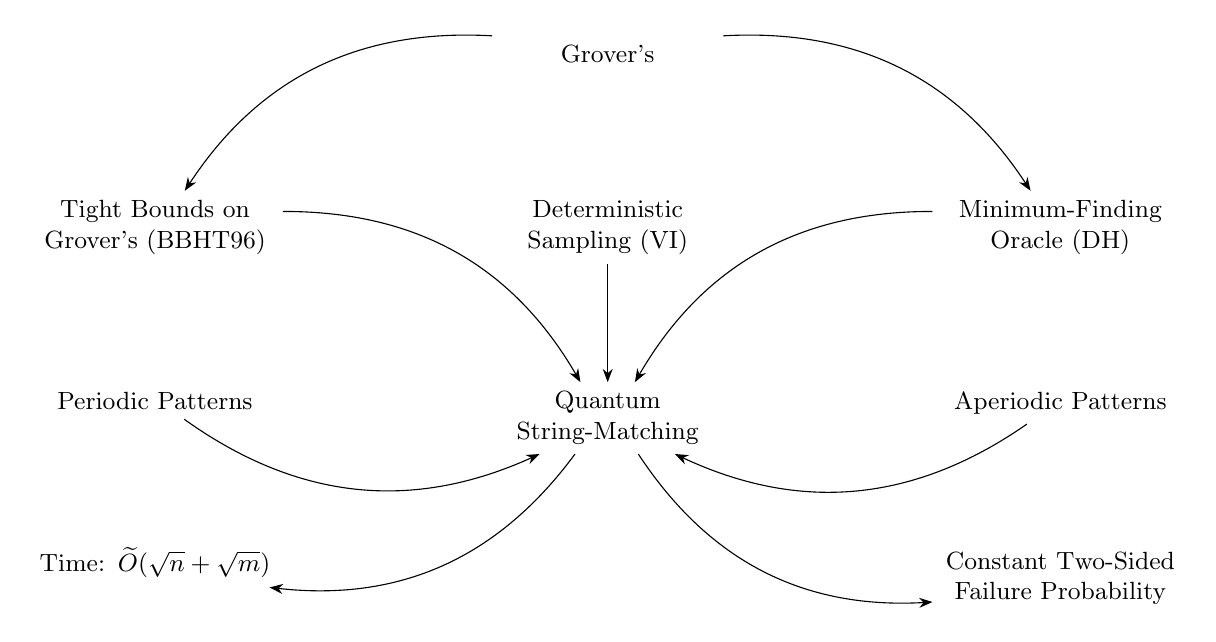
\begin{tikzpicture}[
        scale=0.8,
        >={Stealth[]},
        every node/.style={font=\small, text width=3cm, align=center},
        node distance=1.5cm and 2.5cm
        ]
        % Nodes with plain text only
        \node (proposed)  {Quantum String-Matching};
        \node (vi)       [above=of proposed]      {Deterministic Sampling (VI)};
        \node (grover)   [above=of vi]            {Grover's};
        \node (bbht)     [below left=of grover]   {Tight Bounds on Grover's (BBHT96)};
        \node (dh)       [below right=of grover]  {Minimum-Finding Oracle (DH)};
        \node (aper)     [below=of dh]            {Aperiodic Patterns};
        \node (periodic) [below=of bbht]          {Periodic Patterns};
        \node (time)     [below=of periodic]      {Time: $\widetilde{O}(\sqrt{n}+\sqrt{m})$};
        \node (prob)     [below=of aper]          {Constant Two-Sided Failure Probability};

        % Curvy edges
        \draw[->, bend right]  (grover)   to (bbht);
        \draw[->, bend left]   (grover)   to (dh);
        \draw[->, bend left]   (bbht)     to (proposed);
        \draw[->, bend right]  (dh)       to (proposed);
        \draw[->]              (vi)       to (proposed);
        \draw[->, bend left]   (aper)     to (proposed);
        \draw[->, bend right]  (periodic) to (proposed);
        \draw[->, bend left]   (proposed) to (time);
        \draw[->, bend right]  (proposed) to (prob);
      \end{tikzpicture}%
    }
    \caption{Conceptual dependencies in the $\widetilde{O}(\sqrt{n}+\sqrt{m})$ quantum string-matching algorithm.}
    \label{fig:quantum-string-matching}
  \end{figure}
\end{frame}

\begin{frame}{The Algorithm}
  \begin{figure}
    \centering
    \resizebox{1\textwidth}{!}{%
      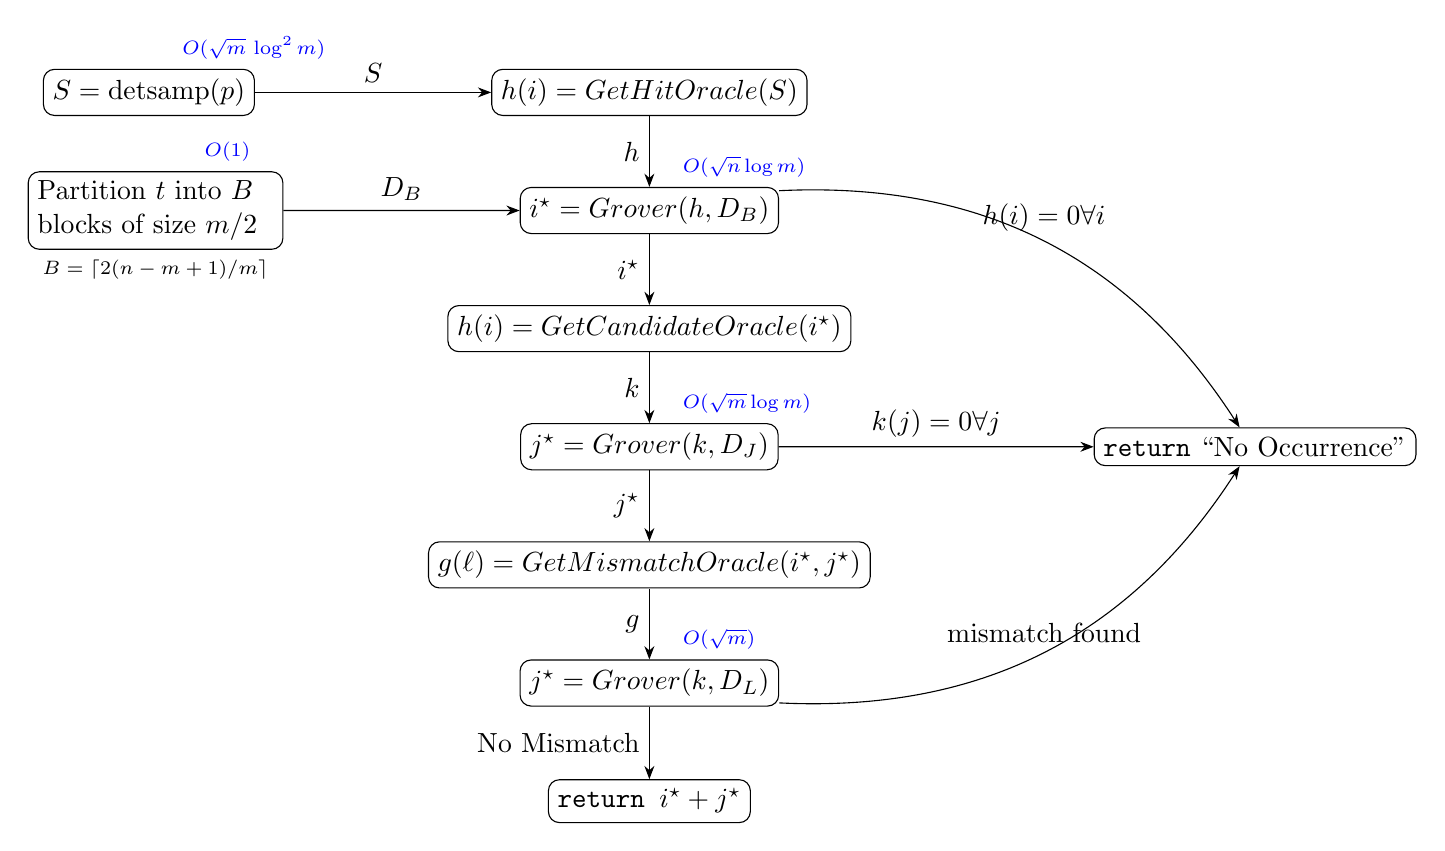
\begin{tikzpicture}[
        scale=0.8,
        >={Stealth[]},
        % every node/.style={font=\small, text width=cm, align=center},
        node distance=1.5cm and 2.5cm
        ]


        \node[draw, rounded corners] (GetHitOracle) {\(h(i) = GetHitOracle(S)\)};

        \node[draw, rounded corners, label=above right:{\scriptsize\textcolor{blue}{ \(O(\sqrt{n} \log m)\)}}]
        (groverh) [below of=GetHitOracle] {\(i^\star = Grover(h, D_B)\)};

        \node[draw, rounded corners] (GetCandidateOracle) [below of=groverh] {\(h(i) = GetCandidateOracle(i^\star)\)};

        \node[draw, rounded corners, label=above right:{\scriptsize\textcolor{blue}{\(O(\sqrt{m} \log m)\)}}]
        (groverk) [below of=GetCandidateOracle] {\(j^\star = Grover(k, D_J)\)};

        \node[draw, rounded corners] (GetMismatchOracle) [below of=groverk] {\(g(\ell) = GetMismatchOracle(i^\star, j^\star)\)};

        \node[draw, rounded corners, label=above right:{\scriptsize \textcolor{blue}{\(O(\sqrt{m})\)}}]
        (groverg) [below of=GetMismatchOracle] {\(j^\star = Grover(k, D_L)\)};

        \node[draw, rounded corners] (return) [below of=groverg] {\texttt{\(\text{return~} i^\star + j^\star\)}};

        \node[draw, rounded corners, label=above right:{\scriptsize \textcolor{blue}{\(O(\sqrt{m}\,\log^2 m)\)}}, left=3cm of GetHitOracle]
        (detsamp) {\(S = \mathrm{detsamp}(p)\)};

        \node[draw, rounded corners, text width=3cm, align=left,
        label=above right:{\scriptsize \textcolor{blue}{\(O(1)\)}},
        label=below:{\scriptsize \(B = \lceil 2(n-m+1)/m \rceil\)},
        left=3cm of groverh]
        (partition)
        {Partition \(t\) into \(B\) blocks of size \(m/2\)};

        \node[draw, rounded corners] (nooccur) [right=4cm of groverk] {\texttt{return} ``No Occurrence''};


        % Edges
        \draw[->] (detsamp.east) to node[midway, above] {\(S\)} (GetHitOracle.west);
        \draw[->] (partition.east) to node[midway, above] {\(D_B\)} (groverh.west);

        \draw[->]  (GetHitOracle) to node[midway, left] {\(h\)} (groverh);
        \draw[->]  (groverh) to node[midway, left] {\(i^\star\)} (GetCandidateOracle);
        \draw[->]  (GetCandidateOracle) to node[midway, left] {\(k\)} (groverk);
        \draw[->]  (groverk) to node[midway, left] {\(j^\star\)} (GetMismatchOracle);
        \draw[->]  (GetMismatchOracle) to node[midway, left] {\(g\)} (groverg);
        \draw[->]  (groverg) to node[midway, left] {No Mismatch} (return);

        \draw[->, bend left]  (groverh) to node[midway, above] {\(h(i) = 0 \forall i\)} (nooccur);
        \draw[->]  (groverk) to node[midway, above] {\(k(j) = 0 \forall j\)} (nooccur);
        \draw[->, bend right]  (groverg) to node[midway, above] {mismatch found} (nooccur);

      \end{tikzpicture}%
    }
    \label{fig:quantum-string-matching-alg}
  \end{figure}
\end{frame}

\section{Preliminaries}

\subsection{Grover's Algorithm}
\begin{frame}{Grover's Algorithm}
  \begin{itemize}
    \item Problem: Given a database of \(N\) elements and oracle \(f(x)=1\) for marked items, find an \(x\) with \(f(x)=1\).
    \item Steps:
          \begin{enumerate}
            \item Initialize \(n\) qubits into uniform superposition over \(N=2^n\) states.
            \item Apply the search oracle to flip the phase of marked states (multiply goal state amplitude by -1).
            \item Apply diffusion operator which reflects all states amplitude across the mean amplitude.
            \item Repeat oracle + diffusion \(\bigl\lfloor\frac{\pi}{4}\sqrt{N}\bigr\rfloor\)
            \item Measure to obtain the marked element with high probability.
          \end{enumerate}
    \item Time Complexity: \(\mathcal{O}\!\bigl(\sqrt{N}\bigr)\).
    \item Why it works: Oracle phase-flips mark targets; diffusion amplifies their amplitudes.
    \item Significance: Core building block for quantum search algorithms.
  \end{itemize}
\end{frame}
\subsection{Tight bounds on quantum searching}
\begin{frame}{BBHT96: Tight bounds on quantum searching}
  \begin{block}{What it is}
    \begin{itemize}
      \item Even when the number of target \(t \ge 1\) items in a database is unknown,
            you can still find a marked item in \(\tilde O(\sqrt{N/t})\) oracle calls.

    \end{itemize}
  \end{block}
  \begin{block}{Why it matters}
    \begin{itemize}
      \item BBHT96 modifies grovers algorithm slightly to function when the number of possible solutions is unknown like in this string matching problem.
    \end{itemize}
  \end{block}
\end{frame}


\subsection{Probablistic Oracles}
\begin{frame}{Probablistic Oracles}
  \begin{block}{What it is}
    \begin{itemize}
      \item We will replace search oracles which flip target states with 100 percent probability with probablistic search oracles which flip target states with 75 percent accuracy
      \item How to preserve accuracy?
      \item We will apply the probabilistic search oracles log(n) times to the current superposition
      \item Afterwards each state will flip or not flip based on what it did in the majority of the log(n) times the probablistic oracle was applied
    \end{itemize}
  \end{block}
\end{frame}

\subsection{\(O(\sqrt{n}\ \sqrt{m})\) time algorithm}
\begin{frame}{String Match in \(O(\sqrt{n}\ \sqrt{m} )\)}
  \begin{block}{Outer Grovers algorthm}
    \begin{itemize}
      \item n = size of text, m = size of pattern, n - m + 1 = comparisons
      \item EX: text = abcdef, pattern = def, n = 6, m = 3.
      \item abc, bcd, cde, and def
      \item \ket{00}: index 0 ... index m-1 (abc)
      \item \ket{01}: index 1 ... index m   (bcd)
      \item \ket{10}: index 2 ... index m+1 (cde)
      \item \ket{11}: index 3 ... index m+2 (def)
      \item Oracle f(i) applies phase kickback if match at position/state i
      \item EX: 1/sqrt(4) \textbf{f(i)} (\ket{00} + \ket{01} + \ket{10} + \ket{11})
      \item States provide position to search oracle
      \item n usually dominates so \(O(\sqrt{n})\) iterations of grovers 
      \item How exactly does the oracle f(i) detect matches?
    \end{itemize}
  \end{block}
\end{frame}

\begin{frame}{String Match in \(O(\sqrt{n}\ \sqrt{m})\) continued}
  \begin{block}{Understanding f(i)}
    \begin{itemize}
      \item Goal: Detect match between two strings
      \item f(i) detects mismatches between its substring and the pattern
      \item Grovers inside f(i) to find mismatch

      
    \end{itemize}
  \end{block}
  \begin{block}{Inner Grovers algorithm}
    \begin{itemize}
      \item States are indices 0,1,...,m-1. Goal state is a k s.t. pattern[k] $\neq$ text[i+k]
      \item Search oracle g(i,j) returns 1 if  pattern[j] $\neq$ text[i+j]
      \item Apply search oracle onto superposition 1/$\sqrt{m}$ g(i,j) $\sum_{j=0}^{m} $\ket{j}
      \item Mismatched states will have their amplitudes increased
      \item After \(O(\sqrt{m})\) iterations measurement will give index of mismatch with high probability
    \end{itemize}
  \end{block}
\end{frame}

\subsection{Deterministic Sampling}
\begin{frame}{Deterministic Sampling}
  \begin{block}{What it is}
    \begin{itemize}
      \item Given an aperiodic pattern \(p\) of length \(m\), and a text block of length \(m/2\), there are \(m/2\) possible alignments.
      \item DS picks \(O(\log m)\) indices in the pattern so that at most one alignment can match all sampled positions.
    \end{itemize}
  \end{block}

  \begin{block}{Steps}
    \begin{enumerate}
      \item Form \(m/2\) ``copies'' of the pattern, each shifted by one position.
      \item Find a column where at least two copies differ.
      \item Select one of the symbols at that column as the sample and discard copies that don't match.
      \item After \(O(\log m)\) rounds, one copy remains; its chosen columns form the sample \(S\).
    \end{enumerate}
  \end{block}

\end{frame}

\begin{frame}{Deterministic Sampling}
  \begin{block}{Why it works}
    \begin{itemize}
      \item Instead of a full pattern check per alignment (\(O(m)\) classically, \(\tilde O(\sqrt m)\) quantum), only \(O(\log m)\) sampled positions are tested.
      \item Only the single surviving alignment requires the expensive full check.
    \end{itemize}
  \end{block}
  \begin{block}{Why it matters}
    \begin{itemize}
      \item Enables the overall quantum string matching to run in \(\tilde O(\sqrt n + \sqrt m)\) by reducing costly \(\sqrt m\) checks to one per text block.
    \end{itemize}
  \end{block}
\end{frame}


\subsection{Minimum Finding Oracle}
\begin{frame}{DH96: Minimum Finding Oracle}
  \begin{block}{What it is}
    \begin{itemize}
      \item Given a database of size \(n\) and a comparison oracle
            that, for any two indices \(i,j\), indicates which element is smaller.
      \item Finds the index of the minimum element in \(O(\sqrt{n})\) time.
      \item Serves as the backbone for all “pick the smallest (or leftmost) index satisfying a condition” steps.
    \end{itemize}
  \end{block}

  \begin{block}{Steps}
    \begin{enumerate}
      \item Pick a random starting position \(k\).
      \item Use Grover's search to find any index \(i\) with \(\text{database}[i] < \text{database}[k]\).
      \item If such an \(i\) is found, set \(k \leftarrow i\) and repeat.
      \item Otherwise, \(k\) is the index of the minimum element.
    \end{enumerate}
  \end{block}
\end{frame}

\begin{frame}{DH96: Minimum Finding Oracle}

  \begin{block}{Why it matters}
    \begin{itemize}
      \item Building the deterministic sampling set:
            Repeatedly eliminate half of the \(m/2\) pattern copies by finding
            the leftmost and rightmost survivor via DH96 in \(O(\sqrt{m}\log m)\) time.
      \item After locating the matching text-block with the \(h(i)\) oracle,
            invoke DH96 over block indices to pinpoint the earliest occurrence,
            preserving the overall \(\tilde{O}(\sqrt{n} + \sqrt{m})\) bound.
    \end{itemize}
  \end{block}
\end{frame}

\section{Quantum String Matching}

\subsection{The Algorithm}
\begin{frame}{The Algorithm (Part 1)}
  \begin{enumerate}
    \item \textbf{Deterministic-Sampling Preprocessing.}
          \begin{itemize}
            \item Run Vishkin's deterministic-sampling on \(p\) of length \(m\) to obtain an \(O(\log m)\)-sized sample set \(S\).
            \item Cost: \(\widetilde O(\sqrt{m}\,\log^2 m)\).
          \end{itemize}
    \item \textbf{Partition the text.}
          \begin{itemize}
            \item Divide the text \(t\) into
                  \[
                    B \;=\; \Bigl\lceil \frac{2(n - m + 1)}{m} \Bigr\rceil
                  \]
                  blocks, each of size \(\approx m/2\).
          \end{itemize}
    \item \textbf{Quantum search for a “hit” block.}
          \begin{itemize}
            \item Define oracle \(h(i)\): tests if block \(i\) has at least one alignment matching on all positions in \(S\) in \(\widetilde O(\sqrt{m}\,\log m)\) time.
            \item Use Grover search over \(i=1,\dots,B\) with oracle \(h\); time \(\widetilde O(\sqrt{n}\,\log m)\). If none found, conclude “no occurrence.”
          \end{itemize}
  \end{enumerate}
\end{frame}

\begin{frame}{The Algorithm (Part 2)}
  \begin{enumerate}
    \setcounter{enumi}{3}
    \item \textbf{Locate surviving alignment in block.}
          \begin{itemize}
            \item Define oracle \(k(i^*,j)\): checks alignment at shift \(j\) in block \(i^*\) on sample \(S\) in \(O(\log m)\) time.
            \item Use Grover search over \(j=0,\dots,\lfloor m/2\rfloor\) with oracle \(k\); time \(\widetilde O(\sqrt{m}\,\log m)\). If none survives, conclude “no occurrence.”
          \end{itemize}
    \item \textbf{Full quantum verification.}
          \begin{itemize}
            \item Run Grover search over \(\ell=1,\dots,m\) with oracle “\(t[i^*+j^*+\ell]\neq p[\ell]\)” to find any mismatch; time \(\widetilde O(\sqrt{m})\).
            \item If no mismatch is found, report occurrence at \(i^*+j^*\); otherwise, conclude “no occurrence.”
          \end{itemize}
  \end{enumerate}
\end{frame}

\subsection{Concerning Periodicity}
\begin{frame}{Concerning Periodicity}
  % discuss periodic vs. aperiodic patterns
  \begin{itemize}
    \item The difference between periodic and aperiodic strings boils down to whether the string consists of a repeating sub-string or not.
    \item Periodicity leads to issues with the deterministic sampling as it means that the unique identification of a match is not guaranteed.
    \item While the algorithm mentioned above processes aperiodic strings, by adding a simple step of pre-processing, the algorithm can also handle periodic string with the same time complexity.

    \item To handle periodic strings, we first find the period $p$ of the repeating pattern. Then, instead of checking every single position in the string for matches, the search space simplifies down to shifts that are multiples of $p$, i.e. checks only occur at every $p$-th position.
  \end{itemize}
\end{frame}

\subsection{Constant Two-Sided Failure Probability}
\begin{frame}{Constant Two-Sided Failure Probability}
  % discuss the importance of the constant two-sided failure probability as mentioned in the paper
  \begin{itemize}
    \item The algorithm, based on the probabilistic Grover's and Quantum Minimum Finding algorithms, has a non-zero probability of:
          \begin{itemize}
            \item failing to find a correct match (false negative), and
            \item finding a match that is incorrect (false positive)
          \end{itemize}

    \item However, these probabilites are constant, allowing them to be driven down to zero by simple repetition.
    \item The $\tilde{O} (\sqrt{n} + \sqrt{m})$ complexity allows the algorithm to be run repeatedly without significant computational costs.
  \end{itemize}
\end{frame}

\subsection{Achieving \texorpdfstring{$\tilde{O}(\sqrt{n} + \sqrt{m})$}{O(sqrt(n)+sqrt(m))}}
\begin{frame}{Achieving \texorpdfstring{$\tilde{O}(\sqrt{n} + \sqrt{m})$}{O(sqrt(n)+sqrt(m))}}
  % bring everything together. Give a run-through of the entire algorithm, putting all the pieces together. 
  So, the final structure of the algorithm is:
  \begin{itemize}
    \item \textbf{Block Search: }Divide a given string into overlapping blocks of $\frac{m}{2}$ length each using Deterministic Sampling. Then use Grover's algorithm to find blocks containing a match. This takes $\tilde{O}(\sqrt{m})$ time per block. For all the blocks, the time complexity becomes:
          \[
            \tilde{O} ( \sqrt{n \over m} ) \times \tilde{O}(\sqrt{m}) = \tilde{O}(\sqrt{n})
          \]
    \item \textbf{Fine Matching: }Once a block is found, use Quantum Minimum Finding over $O(m)$ candidate positions within the block. Thus, the time complexity for this step becomes:
          \[
            \tilde{O}(\sqrt{m})
          \]
  \end{itemize}
  Thus, the overall time complexity becomes:
  \[
    \tilde{O}(\sqrt{n}+\sqrt{m})
  \]

\end{frame}


\section{Conclusion}
\begin{frame}{Conclusion}
  \begin{itemize}
	\item Just like the probability of failure, the probability of success is a constant, and is greater than $\frac12$.
	\item With a highly modular design, the algorithm's modules can be swapped out to accomplish different tasks with similar if not the same time complexity.
	\item A problem left to the reader or to the future is dealing with don't cares in the same time bounds. The main issue is the implementation of quantum convolution using FFT in $\tilde{O}(\sqrt{n})$ time.
	\item The main issue with the implementation of this algorithm is the assumed fast oracle, that is not present in the current tech stack of quantum computers.
  \end{itemize}
\end{frame}

\end{document}